\section{Electrophysiological Measurement Distributions from Experimental Literature}\label{section:nelectro}
Organized, publicly available electrophysiological measurements from single, biological neurons can form an optimization target.
Together, they can be used to parameterize the suite of tests against which a model is optimized.
Optimization makes corresponding model electrophysiological measurements as similar as possible to those observed in biological neurons.

\subsection{NeuroElectro}
One general source of such measurements is The NeuroElectro Project \citep{tripathy2014neuroelectro}, which contains experimental values for 47 distinct electrophysiological measurements across 235 different neuron types.
As with most of the data discussed here, most (but not all) of these measurements were obtained from slice physiology experiments in rodents.
These measurement values were programatically extracted from peer-reviewed journal articles over a $\sim20$ year period from $\sim1990-2012$,
and are made easy to access by an application programming interface (API) that NeuronUnit provides easy access to.
Importantly, the measured values--even for a single neuron type--reflects experiments done in many labs using (in some cases) variable methods.
Therefore, the mean of these values (e.g. the mean input resistance across reported Purkinje cells) averages over heterogeneity across cells within a slice, slices within an animal, animals within a lab, and labs within the field.
The sample size for one measure (e.g. input resistance) may be larger than for another (e.g. resting potential) meaning that they may reflect different subsets of experiments.
With those caveats in mind, NeuroElectro is still the most direct way to get a large number of optimization-constraining data values for most neuron types.

In order to verify that the data from NeuroElectro was plausible and was being captured correctly for the purposes of the work in this thesis, I used the API along with a batch visualization pipeline to  visualize the distributions of electrophysiological measurements and inspect them for a) quality control and b) evidence of multimodality.
Multimodality, meaning multiple peaks in the histogram of a single measurement type for a single cell, could be evidence of a physiological heterogeneity not easily explained by random measurement error.
Two peaks in the histogram, for example, could result from two distinct subclasses of a single nominal neuron type, each with its own (narrower) distribution of the same measurement.
In some instances, the mean and standard deviation alone well-described the measurement distributions, as would be expected for random, normally-distributed measurements of a single cell type under reasonably consistent conditions.
These values were then ``approved" for use in model-fitting.
In other cases, these conditions were not met, as exemplified in the gallery below.

%\begin{comment}
%\begin{figure}
%\centering
%   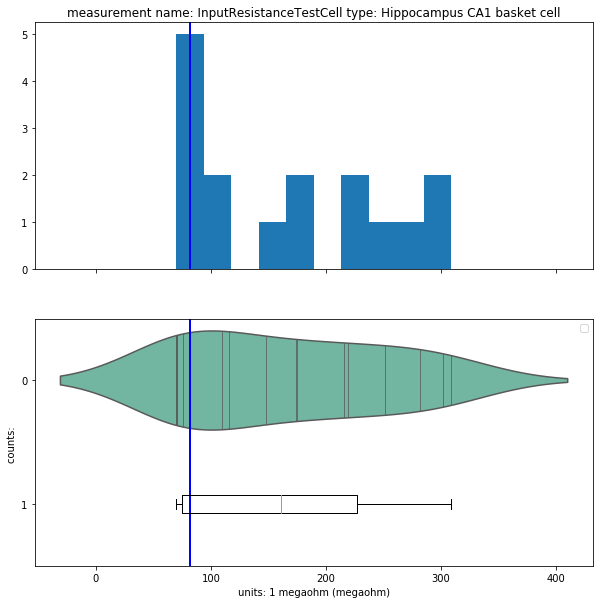
\includegraphics[scale=0.8]{notebooks_converted/needata_thesis_files/needata_thesis_5_5}
%\end{figure}

%\caption{Model parameterization of the brian2 simulator with the customization: interpolated spike height, forced to be above $0mV$}
%
%  \label{fig:sub1}
%\end{subfigure}%
%\begin{figure}
%\centering
%  \includegraphics[scale=0.8]{notebooks_converted/needata_thesis_files/needata_thesis_5_6}
%\end{figure}

%    
%    %\caption{Default model parameterization of the custom written integrator}
%  \label{fig:sub2}
%
%\begin{subfigure}
%  \centering
%      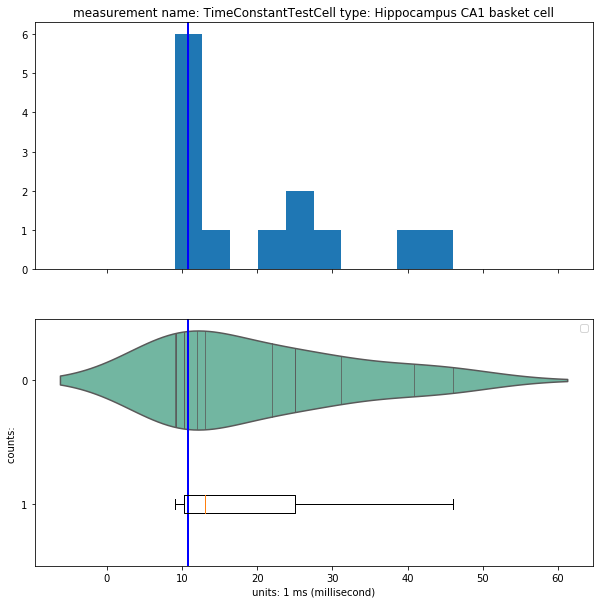
\includegraphics[scale=0.8]{notebooks_converted/needata_thesis_files/needata_thesis_5_7}
%      %\caption{Default model parameterization of the custom written integrator}
%  \label{fig:sub2}
%\end{subfigure}
%
%\caption{Comparison between two Adxaptive Exponential Implementations}
%\label{fig:test}
%\end{center}
%\end{figure}
%
%\end{comment}

%\begin{center}
%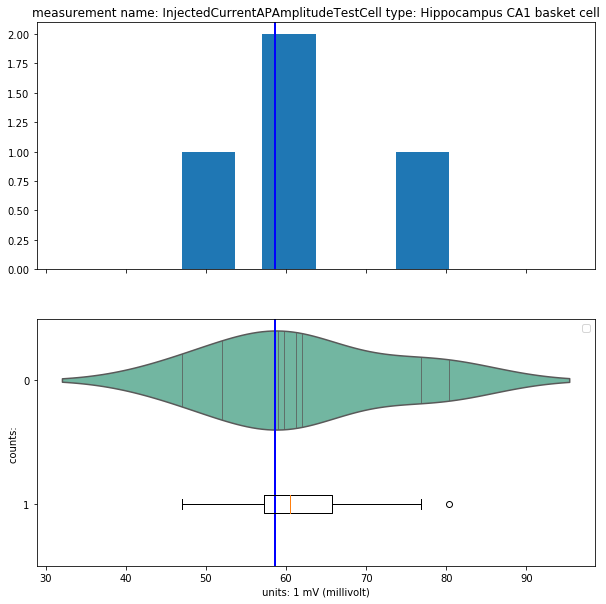
\includegraphics[width=0.7\linewidth]{notebooks_converted/needata_thesis_files/needata_thesis_5_8}
%\end{center}
%
For the majority of NeuroElectro neurons, data sources was uni-modal and well described by a normal distribution. However, as a precaution to ensure data integrity, that a normally distributed data is not a reliable assumption I have humanely identified a minority of distributions that violate this assumption.

%YYYY Done Russell: break this into two plots: one for "good" data and two for "bad" data: of the bad data ones, give one example for bimodal, and one example for skewed.

This analysis was cursory and human driven, although some methods for hypothesis testing that a distribution is bi-modal exist \citep{maechler2013package}, there was not enough time to automate this code. It is estimated, that in all Neuroelectro data sampled here, about $2/3rds$ is well represented by a Gaussian distribution. In the remaining third that was not well represented by a Gaussian reasons for failure included: skewed distribution, bi-modal distribution, uniform distribution, or not enough samples to know inform knowledge of distribution.


\subsubsection{Data well represented by Gaussian normal Distribution}    

\begin{figure} 
    \begin{center}
   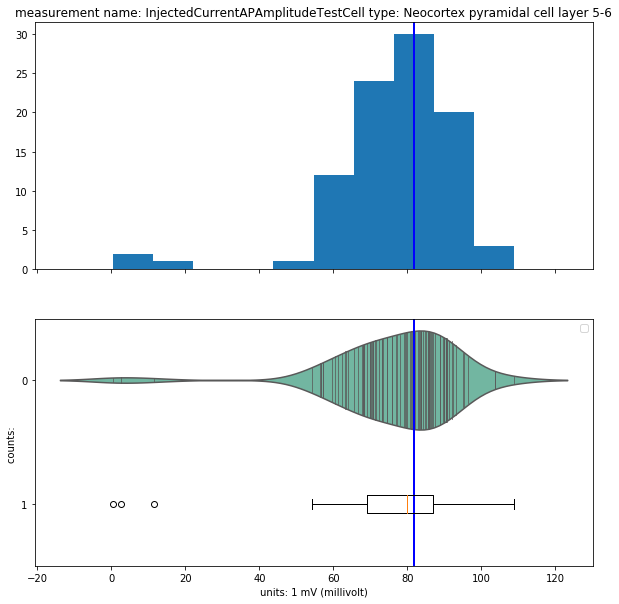
\includegraphics[scale=0.8]{figures/mean_well_served.png}
   \caption[AP Threshold Data Distribution, Layer 5 Pyramidal Cell]{The majority of Neuroelectro data sets were well served by a Gaussian normal distribution. As you can see in this plot the mean is surrounded by a very high density of samples, which slowly thin out with increasing distance from the mean. The distribution is approximately symmetrical, especially for a real data set.}
    \end{center}
\end{figure}   

\begin{figure} 
    \begin{center}
    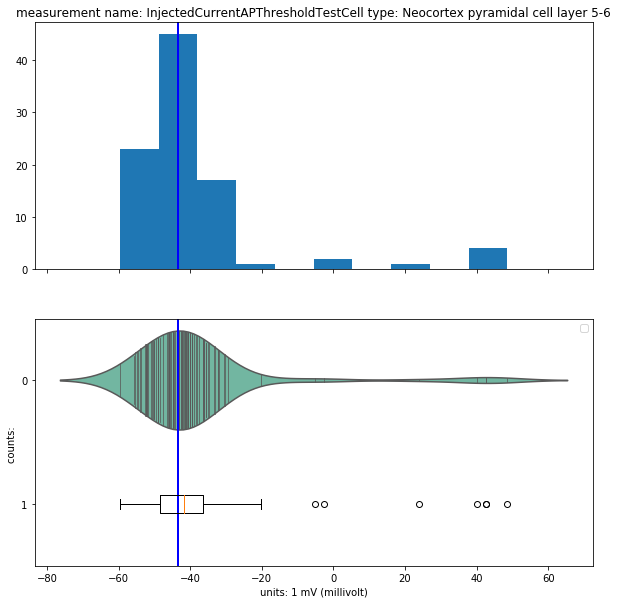
\includegraphics[scale=0.8]{figures/mean_well_served2.png}
    \end{center}
    \caption[AP Amplitude Data Distribution, Layer 5 Pyramidal Cell]{Although the data is skewed to the left and it has outliears. I believe this data distribution is symmetrical enough, to be considered "overall" a normal distribution. In this plot the mean is surrounded by a very high density of samples, which slowly thin out with increasing distance from the mean, although there are a small proportion of outliers these are likely explained by experimental noise.}
\end{figure}   
 
% The distribution is approximately symmetrical, especially for a real data set. 

%YYYY What percentage of ephys features are in each of these categories. I answered this else whare its about 1/3 bad 2/3 good.
\subsubsection{Comparison of Existing Data sets to Normal Distribution}    

\begin{figure} 
    \begin{center}   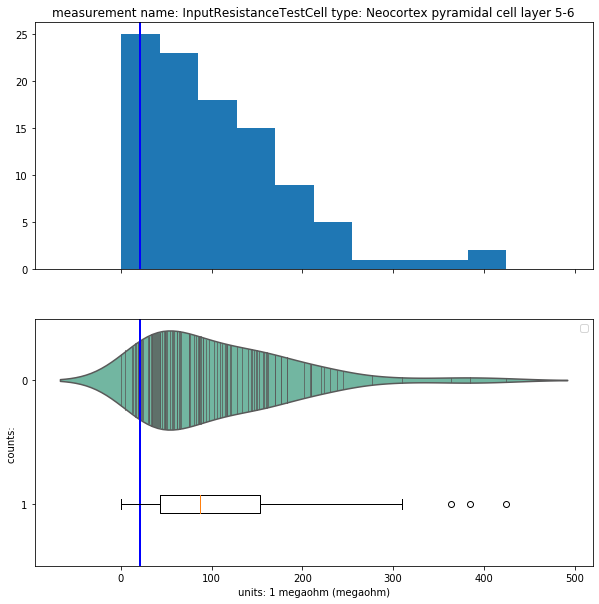
\includegraphics[scale=0.8]{figures/skewed_distribution.png}
    \end{center}
    \caption[Example of skewed NeuroElectro data]{In this distribution of Input Resistance for the Neo-cortical Pyramidal neuron, one can see that values are skewed, and fall off quickly to the right, in this case the median represents the middle of the data better than the mean or the mode.}
\end{figure}   


%\begin{figure} 
%\caption[NeuroElectro data - uniform distribution]{}
%    \begin{center}
%    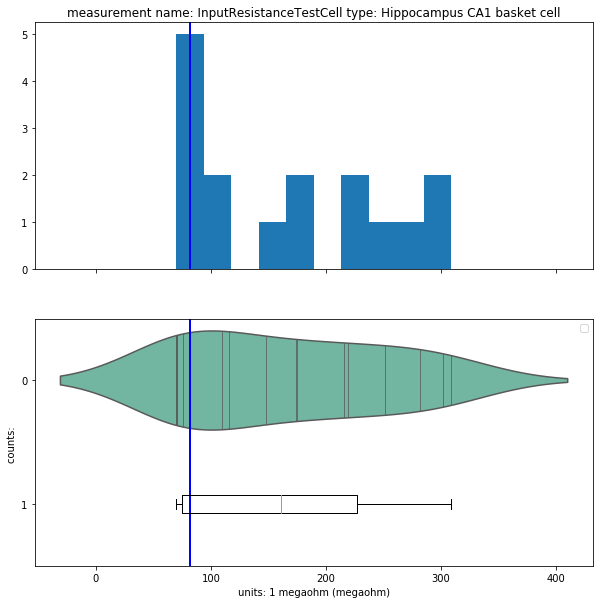
\includegraphics[scale=0.8]{figures/uniform_distribution.png}
%    \end{center}
%\end{figure}       
%%
% Neuronunit code handles under sampled neuroelectro code.
%\begin{figure} 
%\caption[NeuroElectro data - undersampled distribution]{}
%    \begin{center}
%    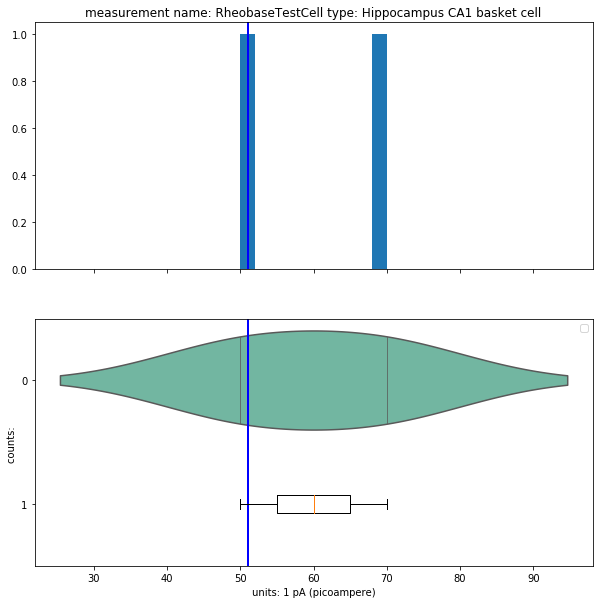
\includegraphics[scale=0.8]{figures/undersampled_distribution.png}
%    \end{center}
%\end{figure}   
%%
    
%\begin{figure} 
%    \begin{center}
%   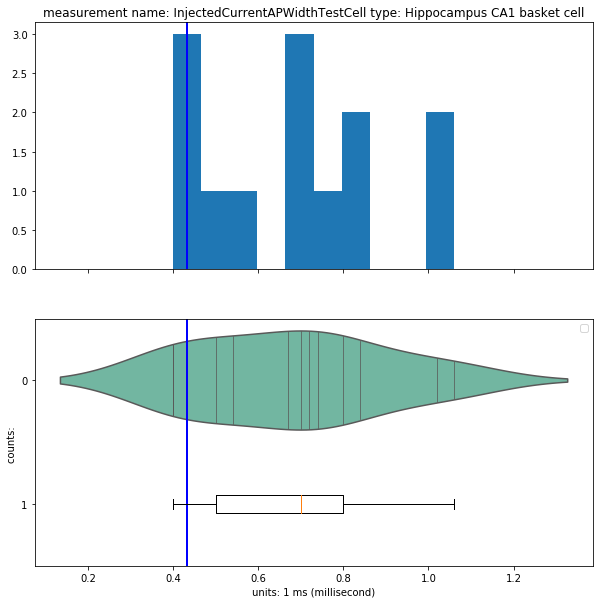
\includegraphics[scale=0.8]{chapters/notebooks_converted/needata_thesis_files/needata_thesis_5_9}
%   \caption{The Action Potential Width of the Hippocampus CA1 basket cell possibly has either an underlying uniform distribution or a multimodal distribution. Since the samples are few, the true distribution is unknown. If the distribution is uniform the gaps in the distribution, that give the histogram a multimodal appearance, as the sample size is lower enough that such gaps may only represent missing samples.}
%    \end{center}
%\end{figure}


%\begin{figure}   
%\begin{center}
%   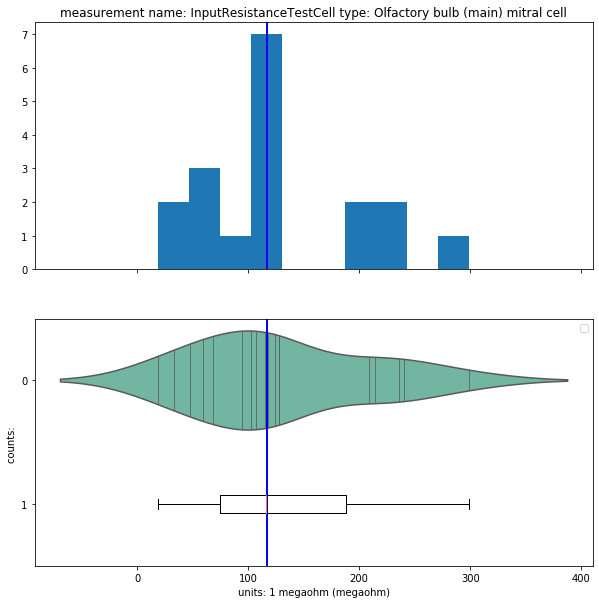
\includegraphics[scale=0.8]{chapters/notebooks_converted/needata_thesis_files/needata_thesis_5_21}
%         \caption[Input Resistance Olfactory Neuron, Perhaps Bimodal]{Input resistance of the Olfactory Mitral cell showed some tendency towards underlying bi-modal distribution, however in the second block of histogram bins, centered around $200-300pA$ only contains approximately $5$ samples. Due to a lack of samples it is also possible to conclude that the data belong to an under sampeled uniform distribution. This data set was important, as one Olfactory neuron test was constructed from this data.}
%\end{center}
%\end{figure}
   
\begin{figure}  
\begin{center}     
  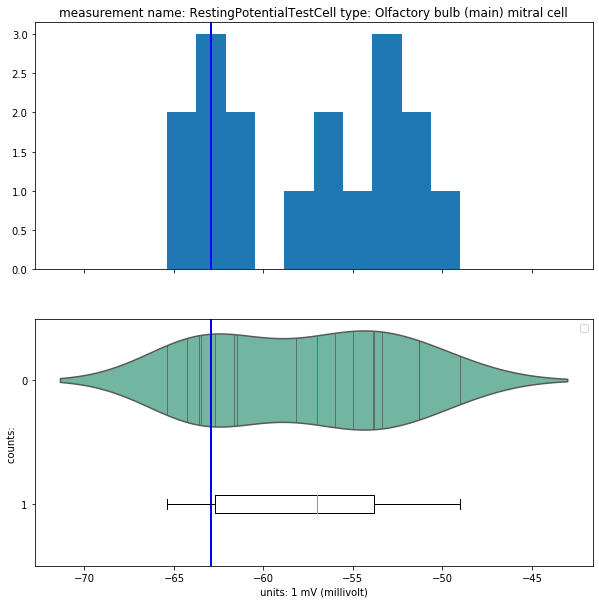
\includegraphics[scale=0.8]{chapters/notebooks_converted/needata_thesis_files/needata_thesis_5_22}
      \caption{Among different measurement sources of neuroelectro data, the resting membrane potential of the Olfactory Mitral cell, showed the greatest tendency of an underlying bi-modal distribution
      In the top panel of this plot we see a binned histogram of Resting membrane potential in the olfactory mitral cell. Although excluded here for considerations of brevity, the input resistance of the olfactory neuron, also perhaps followed a bi-modal or uniform distribution. 
      }
\end{center}     
\end{figure}
%%
% There are plenty of examples of bi-modal distributions in measurements from cells which are not relevant to this work.
%
%\begin{figure}
%  \centering
%  \includegraphics[scale=0.8]{chapters/notebooks_conv%erted/needata_thesis_files/needata_thesis_5_6}
%   \caption{Default model parameterization of the custom written integrator}
%  \label{fig:sub2}
%\end{figure}
%\begin{figure}
%\begin{center}
%includegraphics{chapters/notebooks_converted/needata_thesis_files/needata_thesis_5_13}
%\end{center}
%\end{figure}
    
\begin{figure}
\begin{center}
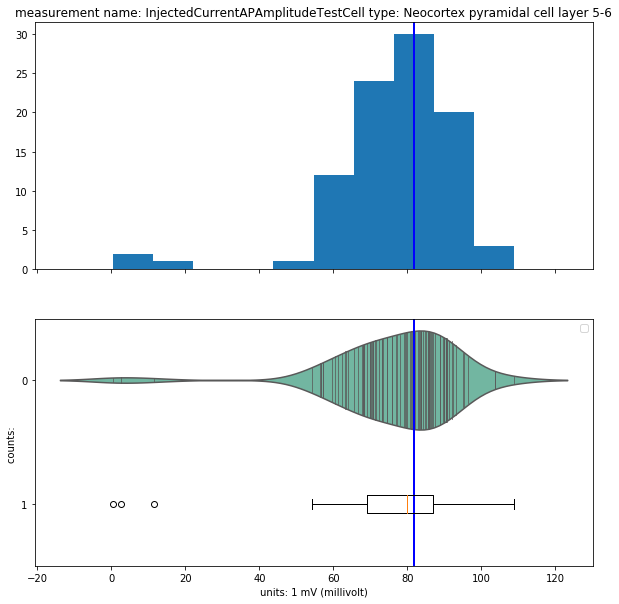
\includegraphics[width=0.7\linewidth]{chapters/notebooks_converted/needata_thesis_files/needata_thesis_5_16}
\end{center}
\end{figure}
\begin{figure}
\begin{center}
     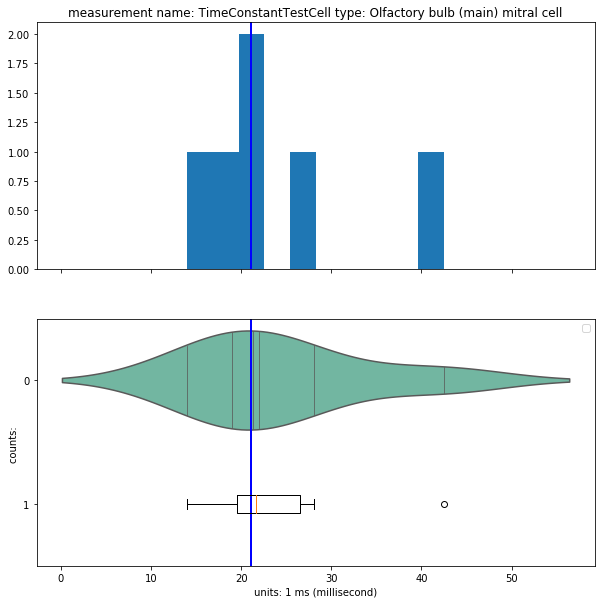
\includegraphics[scale=0.8]{chapters/notebooks_converted/needata_thesis_files/needata_thesis_5_23}
\caption{In the top panel of this plot we see a binned histogram of Neuro electro spike width measurements in the CA1 basket cell Neuron, in the bottom panel we see a violin plot, and a box plot of the same data. In both top and bottom panels, the mode is of the distribution is denoted by a blue vertical line. In this way the mode of the data distribution can be compared to the mean in the box plot. Often modes, and means of the measurements disagree, as they do in the case of CA1 basket cell spike widths. When consulting NeuroElectro measurement, a very common distribution shape is one which is possibly uniform, or multi-modal. It is perhaps obvious but worth noting that a uniform distribution, is not well described by a normal distribution. Under a normal distribution a range of measurement values are equally likely to occur.}
\end{center}
\end{figure}

\subsection{The Allen Institute Cell Types Database}
The data available through NeuroElectro covers a large number of cell types, but recording conditions and measurement algorithms are heterogeneous.
It is unclear if the distribution of measurements across such an ensemble is actually a good summary of any one, real cell.
In order to ensure that reduced models could be optimized against data recorded exclusively from single neurons, I also used the Allen Institute Cell Types Database \citep{celltypes}, a project of the Allen Institute for Brain Science.
This Cell Types database consists of summary physiological, morphological, and histological data for thousands of individual neurons (across a few dozen subtypes) from mouse visual cortex, obtained using patch clamp recordings in slices.
Each experiment is done using exactly the same methods and with the same sequence of stimuli (described in \cite{celltypes}), ensuring not only that models generated using this data are directly comparable, but that each such model is reflective of a single neuron.



The Cell Types Database does provide some limited pre-computed measures of action potential waveform details, however, the data is not organized in a way that makes it is useful for the types of optimization and data analysis I perform,  specifically, I need features computed at on sweeps current injection values that are integer multiples of rheobase. Additionally, pre-computed feature set naturally lack EFEL feature sets which I require, and therefore I need to obtain, through dedicated code.

Because raw data is available through the Cell Types API, it is possible to achieve the required organization by re-computing Allen and EFEL features and I used this to recompute each measurement according to the consistent standard reflected in the NeuronUnit code.
In contrast to NeuroElectro, the Cell Types database also has a great deal more information relevant to the above threshold dynamics of neurons, such as the number and pattern of action potentials they discharge in response to somatically-injected currents much larger than rheobase, or in response to non-square injected currents.
In order to exploit these, I developed several additional NeuronUnit tests, such as: ``time to first spike test" and ``mean AP amplitude test". In principal any EFEL feature, that was measured in Allen Data could be upgraded to a NeuronUnit test, as I created a templates class-code generation method to perform this task. I also created some hard coded EFEL tests on Allen Features too, among the template generated classes, the tests that I re-used for the supra-threshold fits displayed in this work are:

%\begin{figure}
\begin{enumerate}
\item adaptation-index
\item adaptation-index2
\item time-to-first-spike
\item mean-AP-amplitude
\item spike-half-width
\item AHP-depth
\item minimum-voltage
\item peak-voltage
\item time-to-last-spike
\item AHP-depth-abs
\item all-ISI-values
\item voltage-base
\item min-voltage-between-spikes
\item Spikecount
\end{enumerate}

%\label{verbatim:supra-threshold-tests}
%\end{figure}

Below I include some graphs of the many different features utilized in optimization.

\begin{figure}
    \centering
    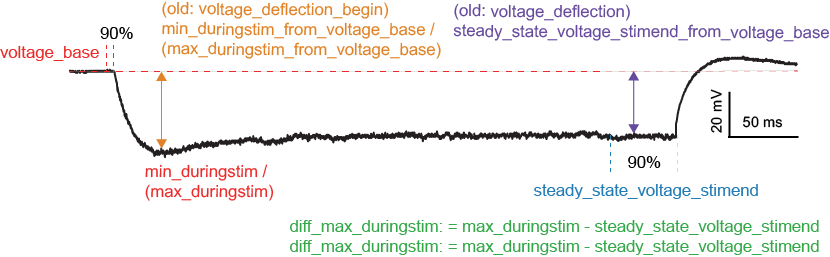
\includegraphics{figures/voltage_features.png}
    \caption[passive membrane properties probed with a negative amplitude current stimulus]{Although applying a negative current stimulus, only tends to activate so called ``passive" ion channels in the membrane, probing the neuron membrane in this way is simple way of ascertaining essential information about neuron membrane resistance and capacitance.  Figures  copied verbatim from https://efel.readthedocs.io/en/latest/eFeatures.html}
    \label{fig:voltage_figures}
\end{figure}





\begin{figure}
    \centering
    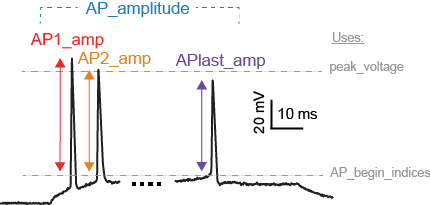
\includegraphics{figures/AP_Amplitude.png}
    \caption[]{When a neuron fires multiple spikes, many features in the waveform are readily measurable, these include, mean AP overshoot, every AP amplitude, wave troughs, spike threshold and after hyperpolarisation potential to name a few}
    \label{fig:features_example}
\end{figure}

\begin{figure}
    \centering
    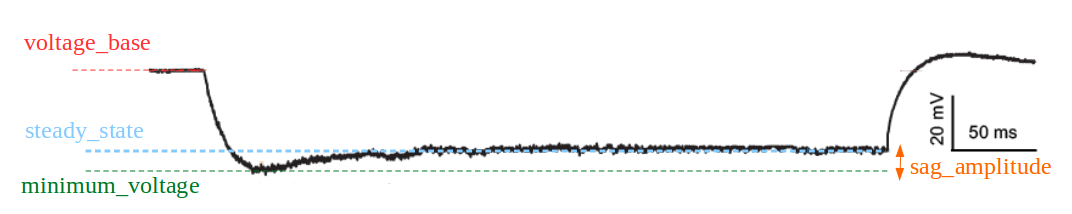
\includegraphics{figures/sag_amplitude}
    \caption{Caption}
    \label{fig:sag_amplitude}
\end{figure}

Two adaption indexs are used to improve the fidelity of adaption measurements, I presume the two different adaption indexs measure adaption in different segments of spike train recordings.

%XXXX Russell, can you list the new tests above.

These tests can be used to assess the agreement between model and biological neurons on suprathreshold dynamics, largely reflected in patterns of spiking such as bursting and adaptation, but also mean spike height, and mean spike width

\subsection{The Blue Brain Project Neocortical Microcircuit Portal}
I also made use of one additional data source, similar in some ways to the Allen Institute Cell Types database but reflecting measurements taken from mouse somatosensory cortex (again in patch-clamp recordings from slices). In terms of the Blue Brain Data set I exclusively used a collection of experiments from animal B-95 \url{http://microcircuits.epfl.ch/#/animal/8ecde7d1-b2d2-11e4-b949-6003088da632}.
Conceptually, this did not add anything new, but it does allow for high-quality optimized models to be produced from another brain region.
However, these data are linked to--and constrain--the on-going Human Brain Project effort to simulated biophysically-detailed multi-compartmental models of the same neurons (and whole neural circuits).
This means that the reduced models produced here can be compared directly to those more detailed models, or that the general NeuronUnit-driven genetic optimization framework developed here can be used to optimize detailed models which should, in principle, be similar to those produced through the larger Human Brain Project effort.

The tests which lead to the best fits in the above threshold experiments, where the tests derived from the above EFEL features applied to NeuronUnit data \ref{fig:supra-threshold-tests}, the measurement type, and the test type did not change between Allen Cell Types, and Blue Brain Data, only the reference data which informed comparison measurements changed.

%YYYY Russell, can you list the new HBP/BBP tests you made above. I believe I have completed this task.


The table below is constitutes a summary of both Neuroelectro and Allen experimental data reports. This data can naturally be reported in tabular form. 

\subsection{The Experimental Measurements}

\begin{table}[ht]
\centering
\resizebox{\textwidth}{!}{
\begin{tabular}{lllllllll}
\toprule
name & Hippocampus CA1 pyramidal cell & Cerebellum Purkinje cell & Neocortex pyramidal cell layer 5-6 &      olf\_mit &      623960880 &      623893177 &      471819401 &      482493761 \\
\midrule
RheobaseTest                   &                      189.24 pA &                680.79 pA &                          213.85 pA &          NaN &        70.0 pA &       190.0 pA &       190.0 pA &        70.0 pA \\
InputResistanceTest            &                    107.08 Mohm &              142.06 Mohm &                        120.67 Mohm &  130.08 Mohm &  241.0 megaohm &  136.0 megaohm &  132.0 megaohm &  132.0 megaohm \\
TimeConstantTest               &                        24.5 ms &                      NaN &                           15.73 ms &     24.48 ms &        23.8 ms &        27.8 ms &        13.8 ms &        24.4 ms \\
CapacitanceTest                &                        89.8 pF &                620.27 pF &                          150.58 pF &    235.75 pF &            NaN &            NaN &            NaN &            NaN \\
RestingPotentialTest           &                      -65.23 mV &                -61.59 mV &                          -68.25 mV &    -58.14 mV &       -65.1 mV &       -77.0 mV &       -77.5 mV &       -71.6 mV \\
InjectedCurrentAPWidthTest     &                        1.32 ms &                  0.41 ms &                            1.21 ms &      1.61 ms &            NaN &            NaN &            NaN &            NaN \\
InjectedCurrentAPAmplitudeTest &                       86.36 mV &                 71.23 mV &                           80.44 mV &      68.4 mV &            NaN &            NaN &            NaN &            NaN \\
InjectedCurrentAPThresholdTest &                       -47.6 mV &                -46.89 mV &                          -42.74 mV &     -38.9 mV &            NaN &            NaN &            NaN &            NaN \\
FITest                         &                            NaN &                      NaN &                         0.05 Hz/pA &          NaN &     0.18 Hz/pA &     0.12 Hz/pA &     0.18 Hz/pA &     0.09 Hz/pA \\
\bottomrule
\end{tabular}}
\end{table}

